
\section{Optimal Monetary Policy}
\label{sec:MonPol}

Our results so far show that BLE generally provides a better model fit than REE for the 3-equation New Keynesian model, with important differences in the estimated structural parameters and the propagation mechanism under BLE and REE. This leaves an important question for the optimal Taylor rule at BLE: how do the optimal values of Taylor rule parameters differ under BLE and REE? In this section we answer this question by considering optimal monetary policy under both calibrated and estimated parameter values.
%Our results so far illustrate that, when BLE and REE are examined under the same set of calibrated parameter values, BLE are characterized by persistence and volatility amplification, with much higher persistence and variance in output gap and inflation compared with REE. As a consequence, there are substantial differences in the estimated parameters and propagation structure when the 3-equation model is evaluated under BLE and REE. This leaves an important question for the optimal Taylor-rule parameters at the BLE. As shown in Boehm and House (2014), at the REE when the output gap and
%inflation are observed without error, it is typically optimal to respond infinitely strongly to observed deviations from the central bank's targets, while with measurement error the optimal Taylor rule coefficients are finite.
%How do the optimal values of Taylor rule parameters differ between the BLE and REE? In this section we try to answer this question by considering optimal monetary policy under both calibrated and estimated parameter values. 
We assume that the central bank wishes to minimize an expected loss function $E[L]$ in terms of the discounted sum of weighted squared inflation, output gap and interest rate
\begin{equation}
E[L]=(1-\vartheta)E\Big[\Sigma_{t=0}^\infty  \vartheta^t[\omega_{\pi} \pi_t^2+\omega_yy_t^2+\omega_r r_t^2] \Big]=\omega_{\pi} \sigma_\pi^2+\omega_y\sigma_y^2+\omega_r\sigma_r^2,\label{varobj}
\end{equation}
where $\omega_i$, $i \in \{\pi,y,r \}$ is the relative weight that the central bank places on inflation, output gap and interest rate respectively. The stabilization objective for inflation and output gap is a standard assumption in the literature, see e.g.  Boehm and House (2014), Evans and Honkapohja (2003) and Woodford (2003). The weight on interest rate variance can be motivated by different interpretations: Woodford (1999) and Giannoni (2014) suggest that it can proxy for welfare costs of transactions and/or an approximation on the zero lower bound on nominal interest rates, while Caplin and Leahy (1996) suggest that it can represent a gradual learning process for the central bank that is uncertain about the consequences of interest rate fluctuations. 

%From the equations (\ref{varyapp}) and (\ref{varpiapp}) in Appendix \ref{acfnkc},
Based on our calculations, the unconditional moments under BLE are given as 
\begin{eqnarray}
\sigma_y^2&=&\frac{\widetilde{g}_1}{(1+\gamma\varphi\phi_\pi+\varphi\phi_y)^2(1-\rho^2)(1-\rho\lambda_1)(1-\rho\lambda_2)(1-\lambda_1^2)(1-\lambda_2^2)(1-\lambda_1\lambda_2)}, \label{varyc}\\
\sigma_\pi^2&=&\frac{\widetilde{g}_2}{(1+\gamma\varphi\phi_\pi+\varphi\phi_y)^2(1-\rho^2)(1-\rho\lambda_1)(1-\rho\lambda_2)(1-\lambda_1^2)(1-\lambda_2^2)(1-\lambda_1\lambda_2)}, \label{varpic}\\
\sigma_r^2&=&\phi_y^2\sigma_y^2+\phi_\pi^2\sigma_\pi^2+2\phi_y\phi_\pi E(y_t\pi_t),\label{varrc}
\end{eqnarray}
where $\widetilde{g}_1$, $\widetilde{g}_2$, $\lambda_1$, $\lambda_2$ are given by the equations (\ref{gyvar}), (\ref{gpivar}), (\ref{lambdatr}) and (\ref{lambdade}), and
\begin{eqnarray*}
E(y_t\pi_t)&=&\Big(-\sigma_y^2\gamma\big(-(1+\gamma\varphi\phi_\pi+\varphi\phi_y)(1+\gamma\varphi\phi_\pi+\varphi\phi_y+\beta_1^2\rho)+\beta_2^4\lambda(1+\gamma\varphi\phi_\pi\\
&&+\varphi\phi_y+\beta_1^2\rho)(\lambda+\gamma\varphi+\lambda\varphi\phi_y)+\beta_2^2\rho[\beta_1^4\lambda+\beta_1^2\lambda\rho(1+\gamma\varphi\phi_\pi+\varphi\phi_y)+\gamma\varphi\\
&&(-1+\lambda \phi_\pi)(1+\gamma\varphi\phi_\pi+\varphi\phi_y)]-\beta_1^2\beta_2^6\lambda^2\rho(\beta_1^2\lambda+\rho(\lambda+\gamma\varphi+\lambda\varphi\phi_y))\big)+\sigma_{\pi}^2\varphi\\
&&\big(-\phi_\pi(1+\gamma\varphi\phi_\pi+\varphi\phi_y)[-\beta_1^4-\beta_1^2\gamma\rho\varphi\phi_\pi+(1+\varphi\phi_y)(1+\gamma\varphi\phi_\pi+\varphi\phi_y)]+\beta_1^2\beta_2^6\lambda\rho\\
&&[-\gamma\varphi(-\beta_1^2+\rho+\rho\varphi\phi_y)+\lambda\rho(\beta_1^4-(1+\varphi\phi_y)^2)]+\beta_2^4\big(\gamma\varphi(1-\beta_1^2\rho+\varphi\phi_y)(1+\gamma\varphi\phi_\pi\\
&&+\varphi\phi_y)+\lambda(-1+\beta_1^2\rho-\varphi(\gamma\phi_\pi+\phi_y))(\beta_1^4-(1+\varphi\phi_y)^2)+\beta_1^2\lambda^2\rho\phi_\pi(-\beta_1^4+\\
&&(1+\varphi\phi_y)^2)\big)+\beta_2^2\rho[-\beta_1^6\lambda\rho\phi_\pi+\beta_1^2\lambda\rho\phi_\pi(1+\varphi\phi_y)(1+\gamma\varphi\phi_\pi+\varphi\phi_y)-(-1+\lambda\phi_\pi)\\
&&(1+\varphi\phi_y)^2(1+\gamma\varphi\phi_\pi+\varphi\phi_y)+\beta_1^4(-1-\varphi(\gamma\phi_\pi+\varphi_y)+\lambda(\phi_\pi+\varphi\phi_\pi\phi_y))]\big)\Big)\Big/  \\
&& \Big((-1+\rho^2)(-1+\beta_1^2\beta_2^2\lambda-\varphi(\gamma\phi_\pi+\phi_y))(1+\beta_1^2\rho(-1+\beta_2^2\lambda\rho)+\gamma\varphi\phi_\pi+\varphi\phi_y\\
&&-\beta_2^2\rho(\lambda+\gamma\varphi+\lambda\varphi\phi_y))\big(\beta_1^4(-1+\beta_2^4\lambda^2)+2\beta_1^2\beta_2^2\gamma\varphi(-1+\lambda\phi_\pi)+(1+\gamma\varphi\phi_\pi+\varphi\phi_y)^2\\
&&-\beta_2^4(\lambda+\gamma\varphi+\lambda\varphi\phi_y)^2\big)\Big).
\end{eqnarray*}
In the following we study the optimal values  $(\phi_y^*, \phi_\pi^*)$ that minimize the central bank's loss function (\ref{varobj}) at the BLE, where $\beta_1^*$ and $\beta_2^*$ are at the BLE   ($\beta_1^*, \beta_2^*$).

\begin{figure}
    \begin{center}
     \includegraphics[width=3.2in]{optpolicy09.eps}
     \end{center}
   \caption{\label{opt09} Optimal policies at the BLE and at the REE. Parameters are: $\lambda=0.99, \varphi=1, \rho=0.5,\gamma=0.04,\sigma_y=1,\sigma_{\pi}=0.5$ and $\omega_y=0.1,\omega_r=0.05$.}
    \end{figure}


\begin{figure}
    \begin{center}
        \mbox{\subfigure[At the BLE ]
        {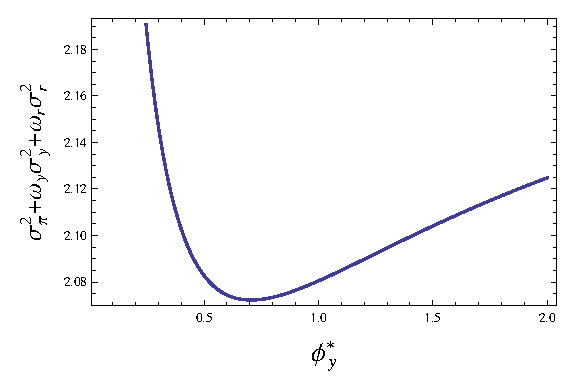
\includegraphics[width=3.2in]{varble09.eps}}\quad
        \subfigure[At the REE]
         {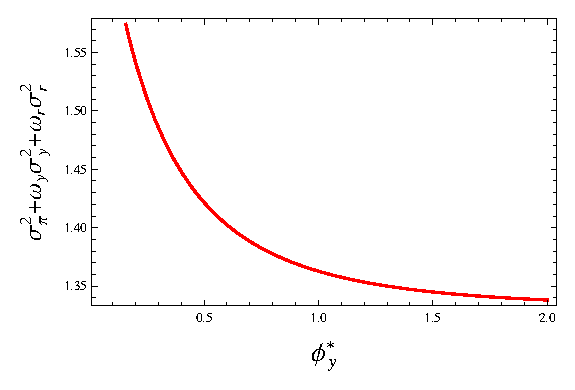
\includegraphics[width=3.2in]{varree09.eps}}}
   \end{center}
   \caption{\label{varopt09} Loss function along the optimal paths $(\phi_y^*, \phi_\pi^*)$ in Figure \ref{opt09} at the BLE (a) and REE (b). Parameters are:  $\lambda=0.99, \varphi=1, \rho=0.5,\gamma=0.04,\sigma_y=1,\sigma_{\pi}=0.5$ and $\omega_y=0.1,\omega_r=0.05$.}
    \end{figure}
    
        We first examine monetary policy under BLE and REE at calibrated parameter values: as before in our calibration exercise, we consider the parameters $\lambda=0.99, \varphi=1, \gamma=0.04, \rho=0.5, \frac{\sigma_{\pi}}{\sigma_y}=0.5$ for both BLE and REE. This ensures that all structural parameters are the same under both specifications, hence the data generating process only differs in terms of the expectation formation rule. The analysis for calibrated parameters provides some insight on how optimal monetary policy under BLE depends on model parameters, particularly the persistence of shocks. As we saw in previous sections, there are important differences in the moments of endogenous variables due to volatility and persistence amplification at BLE. In particular, the implied variances of inflation, output gap and interest rate are different under BLE and REE at these parameter values. Following Woodford (1999) and Giannoni (2014), we normalize the weight on inflation to $\omega_{\pi}=1$. 
        We first focus on a special case with $\omega_y=0.1$ and $\omega_r=0.05$, that is, the central bank places a relatively large weight on inflation and a small one on interest rates. The small weight on interest rates allows us to first focus on the trade-off between inflation and output gap stabilization. We leave the discussion of how optimal policy depends on these policy weight for the more empirically relevant case of estimated parameters. 

    Interestingly, we find that the optimal Taylor rule coefficients $(\phi_y^*, \phi_\pi^*)$ are finite under BLE in this case\footnote{
We first select a policy parameter domain (e.g. $[0,100]\times[1,100]$) and define a lattice with some small step ($e.g. \,\,0.01$). Then for each lattice point $(\phi_y, \phi_\pi)$, we find the BLE $(\beta_1^*(\phi_y, \phi_\pi), \beta_2^*(\phi_y, \phi_\pi))$ and the corresponding central bank's expected loss function $E[L]$ at the BLE. Finally we interpolate the loss function with respect to $(\phi_y, \phi_\pi)$ to find the finite optimal values. It is easy to get analytic expressions of the variances and optimal policy parameters under REE. In contrast, it is impossible to obtain analytic expressions of the optimal policy parameters under BLE and  therefore we have to rely on numerical approximations. We find consistent results using different ways to calculate the variances (i.e. based on (\ref{varyc}) and (\ref{varpic}) or computing the variances as in Appendix \ref{ACFn}).}.
As shown in Figure \ref{opt09}, the corresponding optimal policy is $(\phi_y^*, \phi_\pi^*)=(0.9069, 4.8822)$. This is different from REE, where there is no finite optimal policy except when measurement errors are considered, as shown in Boehm and House (2014)\footnote{The loss function considered in Boehm and House (2014) does not include interest rate variance. Including interest rates in our loss function here does not affect the result that optimal policy at REE does not exit as long as $\omega_r$ remains sufficiently small. Optimal policy becomes finite when $\omega_r$ is sufficiently large, these cases are discussed under the estimated parameter values.}. In fact, from Figure \ref{opt09} it can be seen that in the case $\phi_y^*$ is small enough (i.e. $<0.9069$) the coefficients $\phi_y^*$ and $\phi_\pi^*$ lie on a manifold and the loss function (\ref{varobj}) decreases gradually along the manifold within this region, which is similar to REE but with higher $\phi_\pi^*$. However, for $\phi_y^*>0.9069$, the loss function (\ref{varobj}) starts to increase, while in the REE the loss function (\ref{varobj}) still decreases as shown in Figure~\ref{varopt09}. That is to say, there exist finite optimal Taylor rule coefficients at the BLE, but not at the REE. This is mainly because at the BLE the actual law of motion has higher variance than at the REE for most variables (especially inflation) and minimizing the loss function, i.e. minimizing the weighted variances of output gap and inflation, requires balancing the different responses in terms of policy parameters $(\phi_y, \phi_\pi)$.


  \begin{figure}
    \begin{center}
        \mbox{\subfigure[Optimal policy ]
        {\includegraphics[width=3.2in]{optpolicyrho09.eps}}\quad
        \subfigure[Optimal manifold]
         {\includegraphics[width=3.2in]{optmanifrho.eps}}}
   \end{center}
   \caption{\label{optrho}  Optimal policies at the BLE with respect to $\rho$ (a) and corresponding optimal manifolds for three different $\rho$ (connection points of solid and dotted curves corresponding to finite optimal policies) (b). Parameters are: $\lambda=0.99, \varphi=1, \gamma=0.04,\sigma_y=1,\sigma_{\pi}=0.5$ and $\omega_y=0.1,\omega_r=0.05$.}
    \end{figure}


Next we investigate how optimal monetary policy changes as the persistence of the underlying shocks is varied. At the REE with measurement error the finite coefficients $\phi_y^*$ and $\phi_\pi^*$ increase as the persistence of shocks grows within some range, see Boehm and House (2014). At the BLE, in addition to this, we find that when the persistence of exogenous shocks becomes sufficiently small with $\rho<0.4$, the finite coefficients $\phi_y^*$ and $\phi_\pi^*$ increase in a small region as shown in Figure \ref{optrho}a, before they start decreasing again. Furthermore, Figure \ref{optrho}b suggests that the optimal manifold always moves up as the persistence of shocks $\rho$ grows. The finite optimal policy lies at the point in the optimal manifold connecting the solid and dotted lines in Figure \ref{optrho}b. The location of the optimal point corresponding to finite optimal policies depends on the relative values of variances of inflation, output gap and interest rate. In the case $\rho$ is large enough, the loss function is mainly dominated by the variance of inflation and hence the optimal policy $\phi_{\pi}^*$ grows quickly converging to $\infty$ and the slope of $\frac{\phi_\pi^*}{\phi_y^*}$ converging to a relatively large constant. As $\rho$ becomes smaller, the variance of interest rate starts to play a more dominant role, which leads to smaller values for both ${\phi_\pi^*} $ and ${\phi_y^*}$. The region with small values of $\rho$ is the most relevant for U.S. data since both shock persistence parameters are low at the BLE in our estimation exercises.

%Are the finite optimal policies more aggressive in response to more persistent underlying shocks? At the REE with measurement error the finite coefficients $\phi_y^*$ and $\phi_\pi^*$ increase as the persistence of shocks grows within some range, see Boehm and House (2014). But at the BLE, we find that for relatively large $\rho$ the finite coefficients $\phi_y^*$ and $\phi_\pi^*$ increase as the persistence $\rho$ of shocks grows, while for some smaller range of $\rho$ the finite coefficients $\phi_y^*$ and $\phi_\pi^*$ first increases and then decrease as the persistence $\rho$ of shocks grows, as shown in Figure \ref{optrho}a. Furthermore, Figure \ref{optrho}b suggests that the optimal manifold always moves up as the persistence of shocks $\rho$ grows. The finite optimal policy lies at the point in the optimal manifold connecting the solid and dotted lines in Figure \ref{optrho}b. The location of the optimal point corresponding to finite optimal policies depends on the relative values of variances of output gap and inflation. In the case $\rho$ is large enough, the loss function is mainly dominated by the variance of inflation and hence the optimal policy $\phi_{\pi}^*$ grows quickly converging to $\infty$ and the slope of $\frac{\phi_\pi^*}{\phi_y^*}$ converging to a relatively large constant. For relatively small $\rho$, the effect of $\rho$ with interest variances in the objective function is different from the traditional case without interest variance in the objective function. In any case, the corresponding loss function at the optimal policies at the BLE increases with respect to $\rho$, for example $=\omega\sigma_\pi^2+\omega_y\sigma_y^2+\omega_r\sigma_r^2= 0.5855, 2.0723, 12.8143$ for $\rho=0.35, 0.5, 0.75$, respectively.

%In a similar vein, if the weight on inflation $\omega$ is large enough, the loss function is dominated by the variance of inflation. Figure \ref{optomega}a suggests that the optimal policy is $\phi_\pi^*\to\infty$ and $\phi_y^*\to 0$ for $\omega=1$. Therefore, for large enough $\omega$, finite optimal policy $\phi_\pi^*$ increases while  $\phi_y^*$ decreases as $\omega$ grows, as shown in Figure \ref{optomega}. For small enough $\omega$, the variance of output gap plays a dominant role and hence the optimal manifold increases as $\omega$ grows (see Figure \ref{optomega}b). For a range of  $\omega$ values there exist finite optimal policies. As $\omega$ grows, the finite optimal policy $\phi_\pi^*$ first decreases and then increases, while $\phi_y^*$ decreases  within the range of existence of finite optimal policy.


%Now consider the case $\omega_y=1,\omega_r=0.05$ with all the other parameters as before. In this case, we find that the optimal monetary policies at the BLE are such that  that $\phi_y^*\to \infty$ and $\phi_\pi^*$ lies at a manifold as shown in Figure \ref{optbench}a\footnote{Although the figure only shows the range of $\phi_y^*$ within $[0,2]$, we checked for a larger range  $\phi_y^*\in [0,100]$ and still can not find a finite optimal policy. The corresponding loss function (\ref{varobj}) keeps decreasing even if the decreasing speed is very slow for large $\phi_y^*$. }.
%However, the loss function (\ref{varobj}) along the optimal line varies only little after $\phi_y^*>0.5$, as shown in Figure \ref{optbench}b. In fact, if the policy $\phi_y^*=0.5$, then the corresponding $\phi_\pi^*\approx 1.5$, which suggests that the traditional choice of $(\phi_y, \phi_\pi)=(0.5, 1.5)$ is reasonable and nearly optimal under the BLE framework when the weights on inflation and output gap are equal and the weight on interest rate is small enough. In addition, compared with the REE, all $(\phi_y^*, \phi_\pi^*)$ in the optimal manifold at the BLE satisfy the determinacy condition, which is also a sufficient condition for the existence of BLE, while only for sufficient large $\phi_y^*(>1.35)$ does the corresponding $(\phi_y^*, \phi_\pi^*)$ in the optimal manifold at the REE satisfy the determinacy condition. Furthermore it is easy to see that given $\phi_y^*>1.35$, $\phi_\pi^*$ in the manifold at the BLE is much greater than at the REE. Therefore, although the optimal policy at the BLE with $\omega_y=1,\omega_r=0.05$ is also $\phi_y^*\to \infty$ and $\phi_\pi^*$ lies at a manifold, the optimal manifold at the BLE is much higher than at the REE, which is consistent with higher persistence and higher volatility of inflation compared to the output gap at the BLE.


\begin{figure}
    \begin{center}
        \mbox{\subfigure[Optimal policy ]
        {\includegraphics[width=3.2in]{optpolicyomega05.eps}}\quad
        \subfigure[Optimal manifold]
         {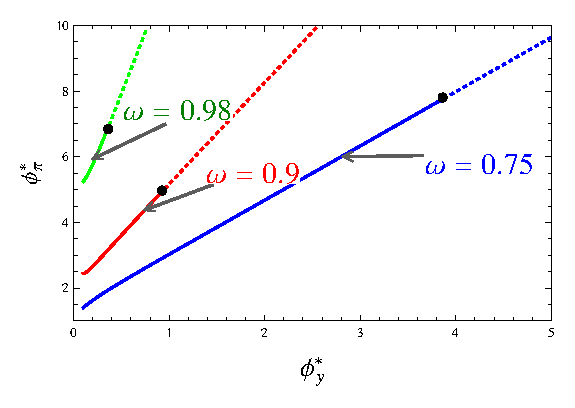
\includegraphics[width=3.2in]{optmanifomega.eps}}}
   \end{center}
   \caption{\label{optomega}  Optimal policies at the BLE with respect to $\omega$ (a) and corresponding optimal manifolds for three different $\omega$ (connection points of solid and dotted curves corresponding to finite optimal policies) (b) with the contemporaneous interest rate rule. Parameters are: $\lambda=0.99, \varphi=1, \gamma=0.04,\frac{\sigma_y}{\sigma_{\pi}}=0.5$ and $\rho=0.5$.}
    \end{figure}
    
%=======================================================================================================   
\begin{sidewaystable}
\small
\begin{tabular}{lll|ll|ll|lllll|lllll}
$\omega_{\pi}$ & $\omega_{y}$ & $\omega_{r}$ & BLE &  & REE &  & BLE &  &  &  &  & REE &  &  &  &  \\
 &  &  & $\phi_y^{*}$ & $\phi_{\pi}^{*}$ & $\phi_y^{*}$ & $\phi_{\pi}^{*}$ & $Var(\pi_t)^{*}$ & $Var(y_t)^{*}$ & $Var(r_t)^{*}$ & $E[L^{*}]$ & $\Delta E[L^{*}]$ & $Var(\pi_t)^{*}$ & $Var(y_t)^{*}$ & $Var(r_t)^{*}$ & $E[L^{*}]$ & $\Delta E[L^{*}]$ \\
\hline
\hline
1 & 0.1 & 0.05 & 3.94 & 3.49 & 2.74 & 4.43 & 0.14 & 0.49 & 1.06 & 0.24 & 58 \% & 0.31 & 0.19 & 1.41 & 0.40 & 27 \%\\
1 & 0.048 & 0.236 & 1.67 & 1.56 & 0.94 & 0.75 & 0.16 & 0.82 & 0.61 & 0.34 & 32 \% & 0.32 & 1.40 & 0.71 & 0.55 & 1 \%\\
\hline
1 & 0.25 & 0 & 15 & 13.33 & 4.35 & 15 & 0.13 & 0.27 & 2.8 & 0.18 & 82 \% & 0.32 & 0.04 & 1.8 & 0.33 & 60 \% \\
1 & 0.20 & 0.05 & 6.67 & 3.94 & 2.64 & 8.51 & 0.14 & 0.35 & 1.45 & 0.28  & 68 \% & 0.32 & 0.07 & 1.61 & 0.41 & 46 \% \\
1 & 0.15 & 0.09 & 3.33 & 2.27 & 1.64 & 3.80 & 0.15 & 0.53 & 0.89 & 0.31  & 58 \% & 0.32 & 0.2 & 1.31 & 0.48 & 31 \% \\
1 & 0.10 & 0.15 & 2.42 & 1.82 & 1.25 & 1.96 & 0.15 & 0.64 & 0.73 & 0.32  & 48  \% & 0.32 & 0.46 & 1.05 & 0.52 & 15 \% \\
1 & 0.05 & 0.2 & 1.82 & 1.67 & 1.06 & 0.87 & 0.16 & 0.77 & 0.64 & 0.32  & 35 \% & 0.32 & 1.19 & 0.77 & 0.53 & 2 \% \\
1 & 0 & 0.25 & 1.21 & 1.67 & 1.07 & 0.01 & 0.16 & 1.05 & 0.58 & 0.31 & 16 \% & 0.30 & 7.91 & 0.45 & 0.41 & 16 \% \\
&  &  &  &  &  &  &  &  &  &  &  &  &  &  &  &  \\
\hline
\hline
$\rho_r=0$ &  &  &  &  &  &  &  &  &  &  &  &  &  &  &  &  \\
$\omega_{\pi}$ & $\omega_{y}$ & $\omega_{r}$ & BLE &  & REE &  & BLE &  &  &  &  & REE &  &  &  &  \\
 &  &  & $\phi_y^{*}$ & $\phi_{\pi}^{*}$ & $\phi_y^{*}$ & $\phi_{\pi}^{*}$ & $Var(\pi_t)^{*}$ & $Var(y_t)^{*}$ & $Var(r_t)^{*}$ & $E[L^{*}]$ & $\Delta E[L^{*}]$ & $Var(\pi_t)^{*}$ & $Var(y_t)^{*}$ & $Var(r_t)^{*}$ & $E[L^{*}]$ & $\Delta E[L^{*}]$ \\
 \hline
1 & 0.1 & 0.05 & 1.21 & 1.67 & 2.17 & 4.91 & 0.14 & 0.47 & 0.97 & 0.24 & 59 \% & 0.32 & 0.09 & 2.01 & 0.43 & 21 \% \\
1 & 0.048 & 0.236 & 0.46 & 0.91 & 0.38 & 0.49 & 0.16 & 1.03 & 0.41 & 0.30 & 40 \% & 0.35 & 2.34 & 0.78 & 0.64 &-16 \% \\
\hline
1 & 0.25 & 0 & 15 & 8.79 & 3.99 & 15 & 0.13 & 0.051 & 4.65 & 0.15 & 85 \% & 0.32 & 0.02 & 2.25 & 0.33 & 61 \% \\
1 & 0.20 & 0.05 & 2.12 & 1.67 & 2.31 & 10.36 & 0.14 & 0.28 & 1.46 & 0.27 & 69 \% & 0.32 & 0.023 & 2.18 & 0.43 & 43 \% \\
1 & 0.15 & 0.09 & 1.06 & 1.21 & 1.01 & 3.75 & 0.15 & 0.52 & 0.79 & 0.30 & 60 \% & 0.33 & 0.12 & 1.93 & 0.54 & 22 \% \\
1 & 0.10 & 0.15 & 0.76 & 1.06 & 0.62 & 1.62 & 0.15 & 0.68 & 0.59 & 0.31 & 59 \%  & 0.33 & 0.47 & 1.53 & 0.61 & 1 \% \\
1 & 0.05 & 0.20 & 0.46 & 1.06 & 0.45 & 0.60 & 0.15 & 1.02 & 0.44 & 0.29 & 41 \% & 0.35 & 1.84 & 0.92 & 0.62 &-15 \% \\
1 & 0 & 0.25 & 0.30 & 1.06 & 0.99 & 0.01 & 0.16 & 1.41 & 0.38 & 0.25 & 31 \% & 0.35 & 7.93 & 0.43 & 0.45 & 3 \%
\end{tabular}
 \caption{\label{optpolicy_table} Optimal Taylor rules and some key statistics at BLE and REE: top panel shows the results under the estimated parameter values in each case, while the bottom panel shows the same results without interest rate smoothing. $E[L^{*}]$ shows the loss function value at the optimal plan, while $\Delta E[L^{*}]$ shows the percentage improvement at the optimal plan relative to the loss function at the estimated parameters.  }

\end{sidewaystable}


 %pdf versions are having trouble with the printer...
\begin{figure}[!h]
  \begin{center}
 
    
    \subfigure[$\phi_y^{*}$ at BLE.]{\includegraphics[scale=0.25]{optPolicy_BLE_est_phiY.jpeg}}
    \subfigure[$\phi_{\pi}^{*}$ at BLE.]{\includegraphics[scale=0.25]{optPolicy_BLE_est_phiPi.jpeg}}\\
    \subfigure[$\phi_y^{*}$ at REE.]{\includegraphics[scale=0.25]{optPolicy_REE_est_phiY.jpeg}}
    \subfigure[$\phi_{\pi}^{*}$ at REE.]{\includegraphics[scale=0.25]{optPolicy_REE_est_phiPi.jpeg}}
    \end{center}
 \caption{\label{optpolicy_est_figures}  Optimal policies at BLE and REE as a function of  $\omega_y$ and $\omega_r$ over the range $[0, 0.25]$. The upper and lower boundaries are 0 and 15 for the optimal parameters.}
    
\end{figure}


\begin{figure}[!h]
    \begin{center}
  
    
     \mbox{\subfigure[$\phi_{\pi}^{*}$ as a function of $\frac{\omega_r}{\omega_y}$.]{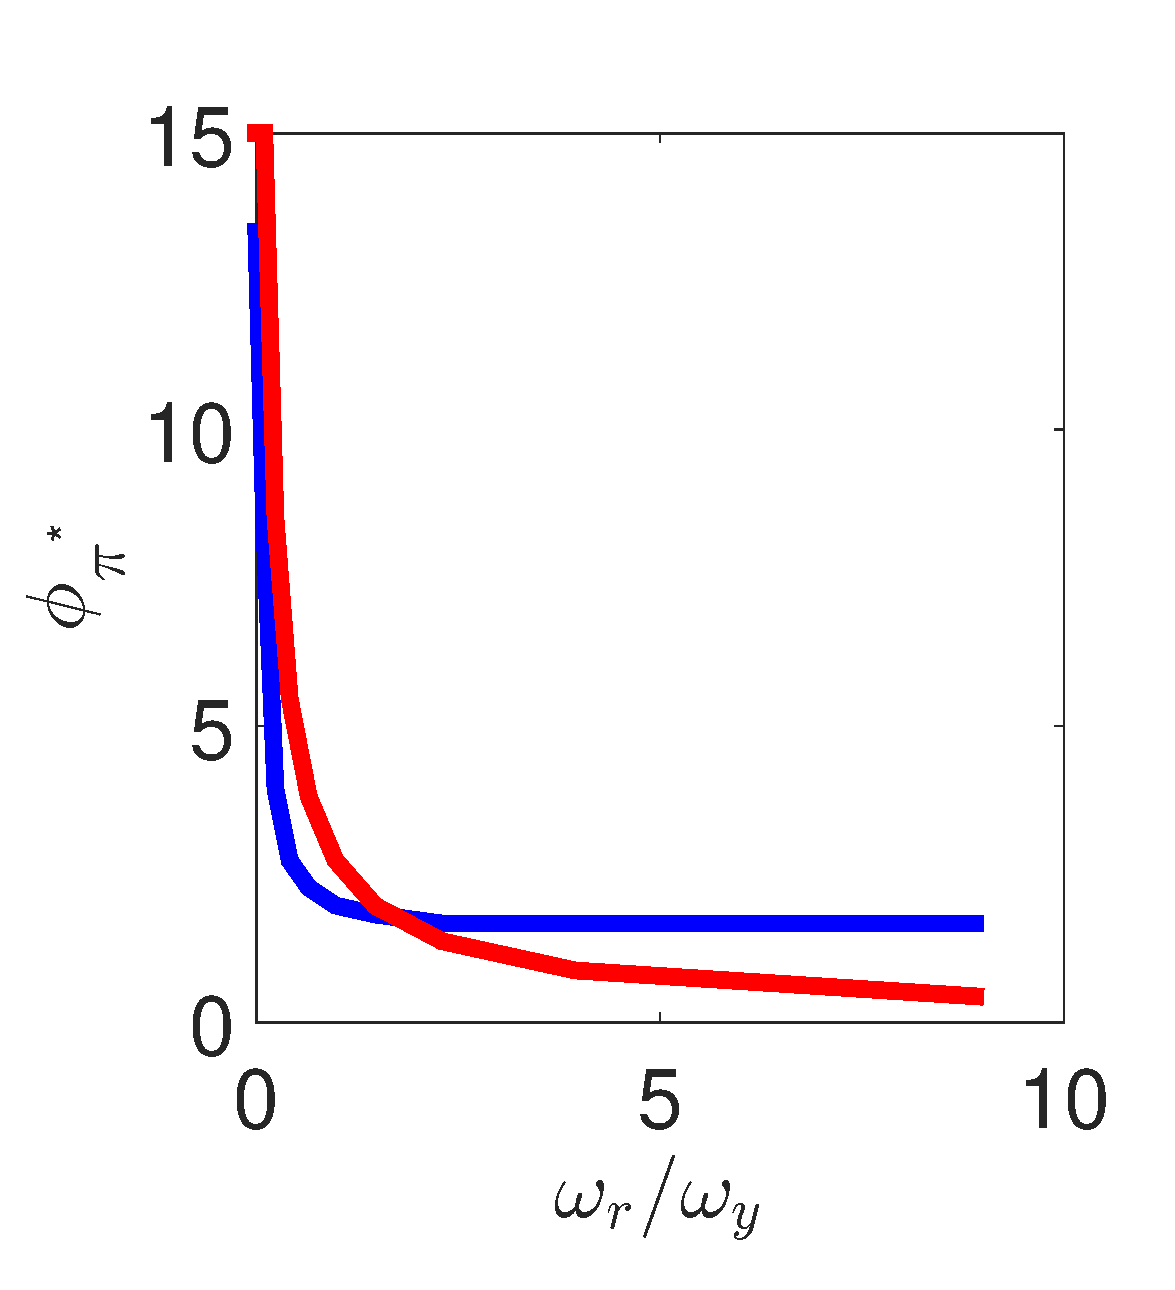
\includegraphics[scale=0.25]{opt_policy_ratios_phiPi.pdf}}} \hspace{5 mm}
      \mbox{\subfigure[$\phi_{y}^{*}$ as a function of  $\frac{\omega_r}{\omega_y}$.]{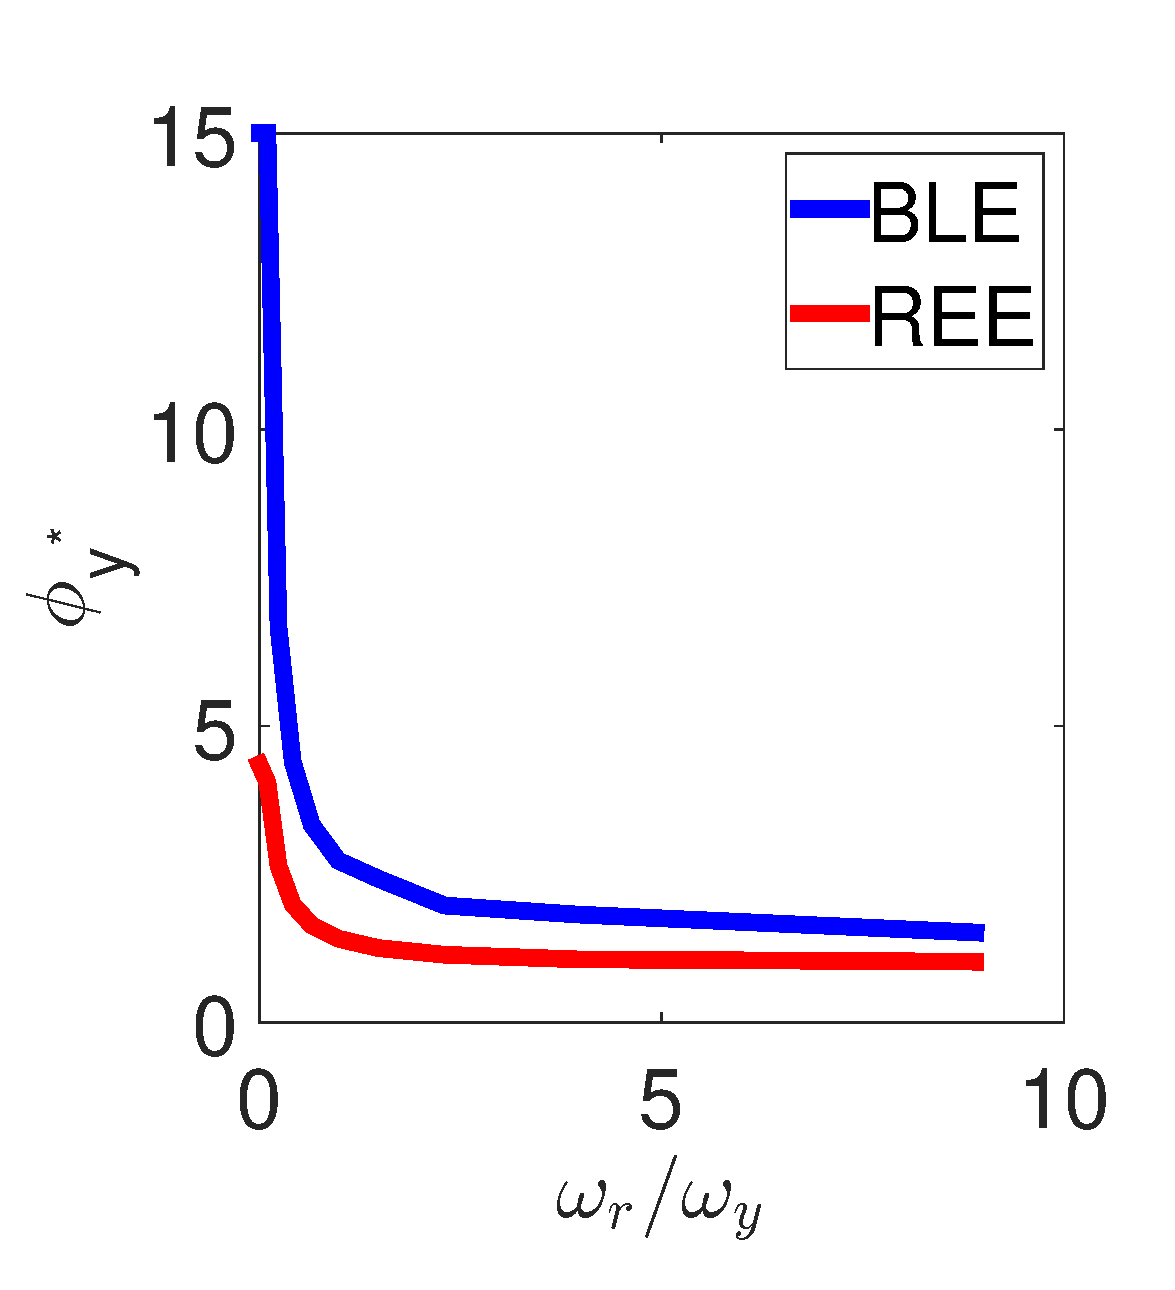
\includegraphics[scale=0.25]{opt_policy_ratios_phiY.pdf}}}\\
      \mbox{\subfigure[IRF of output gap.]{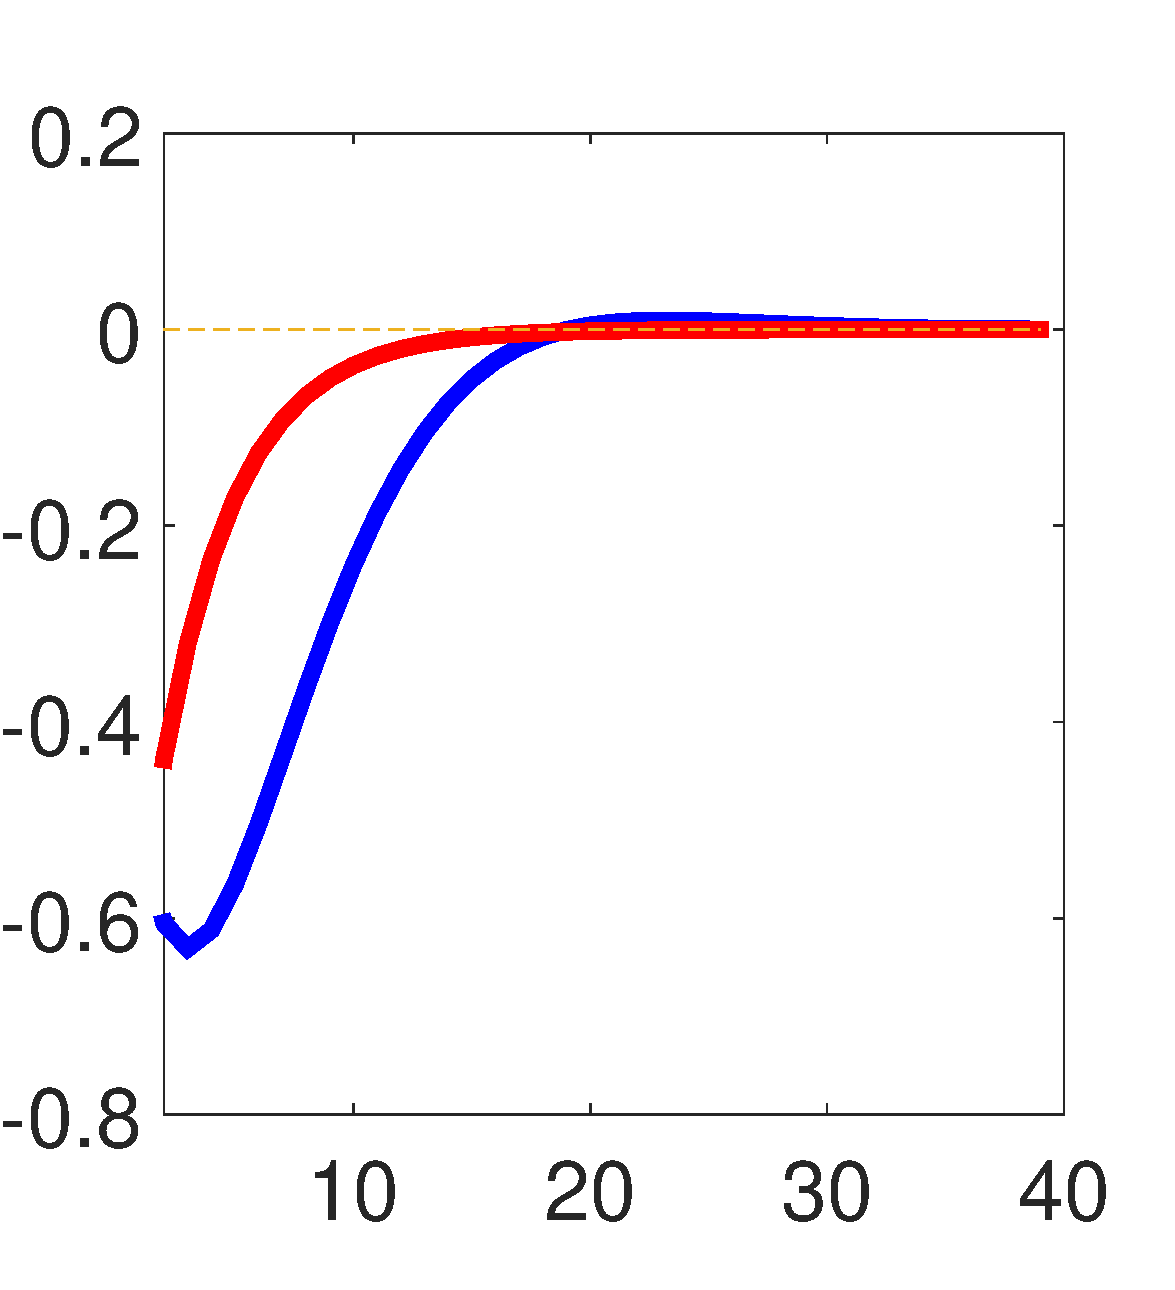
\includegraphics[scale=0.25]{nkpc_irfs_y.pdf} }} \hspace{5 mm}
\mbox{\subfigure[IRF of inflation.]{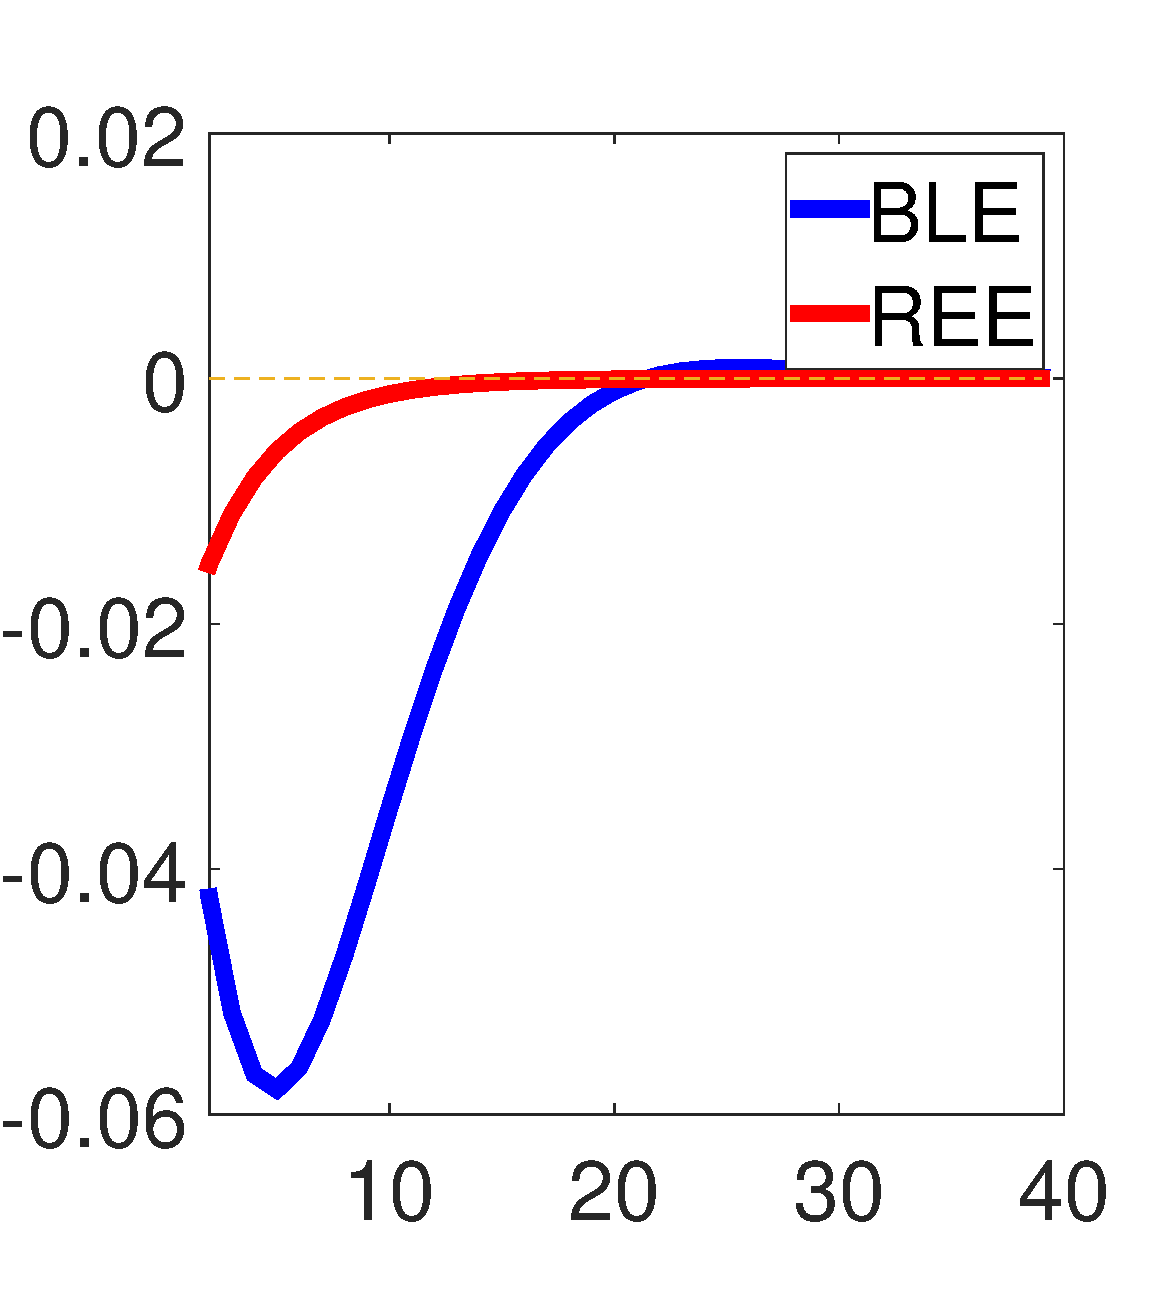
\includegraphics[scale=0.25]{nkpc_irfs_pi.pdf} }}
  \caption{\label{nkpc_irfs} Top panel: changes in optimal parameters as a ratio of weights on interest rates and output gap. Bottom panel: impulse response functions of output gap and inflation to a one standard deviation monetary policy shock.}
    \end{center}
\end{figure}

\vspace{3 mm}


Our analysis so far shows that optimal policy exists under BLE for the calibrated parameters and that the optimal rule $(\phi_{y}^{*},\phi_{\pi}^{*})$ is sensitive to the persistence of exogenous shocks. We next investigate optimal monetary policy for the more empirically relevant case of estimated parameters. In this case the underlying structural parameters are different at BLE and REE, but the variances of inflation, output gap and interest rate are close under these two specifications. In particular, given the estimated parameter values and our benchmark policy weights of $(\omega_y, \omega_r)=(0.1,0.05)$, the expected loss function $E[L]$ is $0.57$ at BLE and $0.55$ at REE\footnote{Our analysis with calibrated parameter values is based on the expressions (\ref{varpic})-(\ref{varrc}). These expressions are no longer applicable for the estimated version of the model since it also includes an interest rate smoothing parameter, and the assumption of same persistence for the exogenous shocks is relaxed. Rather, we use the (different) estimated shock persistence parameters. Therefore we proceed by computing the BLE and the associated variances for each value of policy parameters using the Iterative E-stability algorithm.}. This ensures that the starting point for the loss functions is similar at BLE and REE, unlike the previous case with calibrated parameters.

For this exercise, we limit our attention to Taylor parameters $\phi_y$ and $\phi_{\pi}$ over the range $[0,15]$. Figure \ref{optpolicy_est_figures} shows the optimal rules at BLE and REE for values between $[0, 0.25]$ for $\omega_y$ and $\omega_r$, with $\omega_{\pi}$ fixed at 1. The first result that stands out is, in this case the optimal monetary policy exists not only at BLE, but also at REE for a wide range of policy weights. This difference at REE with estimated parameters arises from the highly persistent shocks and flatter Phillips curve compared with the calibrated parameters, which introduces a larger trade-off between inflation and output gap stabilization, thereby leading to a finite optimal policy for a wide range of policy weights. This additional result allows us to compare how the optimal rules differ under BLE and REE.

Table \ref{optpolicy_est_figures} shows the optimal Taylor rules for several pairs of $(\omega_y,\omega_r)$, along with some key statistics at BLE and REE. The first two rows show our benchmark calibration of $(0.1,0.05)$, while the second row includes a calibration of $(0.048,0.236)$ as in Woodford (1999) and Giannoni (2014). The remaining columns start with the corner case of $(0.25,0)$ with no weight on interest rates, and gradually move to the other corner case of $(0,0.25)$ with no weight on output gap. Several observations stand out from the table: both at BLE and REE, when $\omega_r=0$, there is no optimal policy over the range that we consider\footnote{An optimal policy with larger parameters exists at both BLE and REE if we relax the upper bound of 15. We omit these cases from our discussion here.}. As $\omega_r$ increases, the optimal rules at both BLE and REE decrease to plausible values. An immediate result that stands out is that, $\phi_{\pi}^{*}$ is less sensitive to the policy weights at BLE, while $\phi_y^{*}$ is less sensitive at REE. In other words, optimal monetary policy at REE responds to changes in policy weights mainly through $\phi_{\pi}^{*}$, while optimal monetary policy at BLE responds to these changes through $\phi_y^{*}$. A similar effect can also be seen in Figure \ref{nkpc_irfs}a and \ref{nkpc_irfs}b, which shows the optimal parameters as a function of the ratio of policy weights $\frac{\omega_r}{\omega_y}$. This result is driven by the fact that both estimates of  $\frac{1}{\varphi}$ and $\gamma$ are larger under BLE, which leads to a stronger transmission channel of monetary policy. This in turn allows interest rate changes to have a larger impact on output gap, and a stronger feedback from output gap to inflation at BLE. The stronger transmission channel at BLE is also evident from Figure \ref{nkpc_irfs}c and \ref{nkpc_irfs}d, which shows the impulse responses of inflation and output gap to a monetary policy shock of the same size\footnote{The shock size is one standard deviation at the estimated parameter values for each case, which is the same under BLE and REE with $0.29$.}. Both the initial impact, as well as the cumulative impact of the shock are larger under BLE. Furthermore the shock takes several quarters to reach its full impact under BLE, leading to hump-shaped responses for both inflation and output gap. This is consistent with previous studies in the literature, where a contractionary monetary policy shock typically leads to hump-shaped decreases in output and inflation with peaks after one to two years; see e.g. Leeper et al. (1996) and Christiano et al. (1999). This effect is absent at REE, and it shows that the persistence amplification at BLE is also indirectly reflected in the system's response to an exogenous monetary policy shock. As a consequence of this stronger transmission channel, inflation is more responsive to changes in interest rate at BLE, which leads to smaller fluctuations in $\phi_{\pi}^{*}$. In particular for sufficiently large $\omega_r$, $\phi_{\pi}^{*}$ stabilizes around 1.67 at BLE, which is the close to the standard value of inflation reaction associated with the Taylor rule. Using Woodford (1999) calibration of $(\omega_y,\omega_r)=(0.048,0.236)$, the optimal rule at BLE is given by $(\phi_y^{*},\phi_{\pi}^{*})=(1.67,1.56)$, while the optimal rule at REE falls into the indeterminacy region with $(\phi_y^{*},\phi_{\pi}^{*})=(0.94,0.75)$.

The column $E[L^{*}]$ in Table \ref{optpolicy_est_figures} shows the value of the loss function at the optimal rule for a given pair of weights $(\omega_y,\omega_r)$, and $\Delta E[L^{*}]$ shows the percentage improvement at the optimal rule relative to the loss function at the estimated parameters. It is readily seen that the values for $\Delta E[L^{*}]$ obtained at BLE are generally larger than REE. This is again a consequence of the stronger transmission channel at BLE, which allows monetary policy to have a larger influence in stabilizing the economy. In particular, the optimal variance of inflation obtained at BLE is typically less than half of the optimal variance of inflation at REE. 

In our analysis above, the optimal parameters are inevitably influenced by the degree of interest rate smoothing $\rho_r$. Since this parameter is estimated at different values at BLE and REE with $0.85$ and $0.8$ respectively, we also examine optimal policies at BLE and REE when $\rho_r=0$, which is illustrated at the bottom panel of Table \ref{optpolicy_table}. It is readily seen that our results continue to hold in this case: $\phi_{\pi}^{*}$ is less sensitive and $\phi_y^{*}$ is more sensitive at BLE to changes in policy weights, and the percentage changes $\Delta E[L^{*}]$ in the loss function are generally larger compared to REE. The only difference with the previous case is that the optimal parameters are generally smaller at both BLE and REE, which is expected since shutting off $\rho_r$ allows for larger movements in interest rates, which in turn leads to smaller optimal parameters. This final exercise also reveals that, interest rate smoothing is typically welfare improving at REE, while this is never the case at BLE. $E[L^{*}]$ is uniformly smaller and $ \Delta E[L^{*}]$ uniformly larger at BLE when interest rate smoothing is shut off, while the opposite holds at REE. The result for REE is well-known from Woodford (1999), where a commitment to interest rate smoothing can have a stabilizing effect with forward-looking agents who anticipate and take into account future changes in interest rate. This is different than a BLE with backward-looking agents, where such a commitment does not have a stabilizing effect since agents are unaware of the commitment or do not take it into account when forming their expectations. Overall, these results show that optimal monetary policy at BLE can differ from that at REE in important ways. Particularly, what is optimal under REE may be far from optimal under BLE.




%\begin{figure}
%\centering
%\caption{Impulse responses to a monetary policy shock of one standard deviation. The blue and red lines show the responses under BLE and REE respectively.}
%\label{imp_resp}
%\end{figure}
             
 %We close this section with an illustration of how multiplicity of equilibria can arise under BLE when monetary policy parameters are varied. In all calibration and estimation exercises that we discussed so far, the underlying BLE is unique. However, multiple stable BLE can arise for certain combinations of parameter values. One such case can be observed when we set the parameter values to their CBO-based output gap estimations as given in Table \ref{nkm_alt_gap}, and vary the values of monetary policy parameters. 
%\begin{figure}
%\centering        
%             \mbox{\subfigure[Variances $\sigma_y^2$ and $\sigma_{\pi}^2 $ w.r.t. $\phi_{y}$]{\includegraphics[scale=0.19]{phi_y_variance.pdf}   }} 
% \mbox{\subfigure[Variances $\sigma_y^2$ and $\sigma_{\pi}^2 $ w.r.t. $\phi_{y}$]{\includegraphics[scale=0.19]{phi_pi_variance.pdf}}} \\  
%            \caption{Optimal Policy under BLE and REE at the estimated parameter values.}
%            \label{mult_eqm}
%\end{figure}  
%In this case the estimated Philips curve slope $\gamma$ is smaller at $0.024$ compared with our benchmark estimation with $\gamma=0.035$. Figure \ref{optim_est} illustrates how inflation and output gap variances change as we vary the monetary policy coefficients $\phi_y \in [0.25, 0.5]$ and $\phi_{\pi} \in [1,1.75]$ in this case. While the change in variances follow the same overall pattern as in the benchmark case, we observe two co-existing E-stable BLE over a small range of parameter values. The underlying BLE is unique at the estimated parameter values, but as the reaction coefficients become smaller, with $\phi_y<0.33$ or $\phi_{\pi}<1.3$, another BLE with higher variance and higher persistence for both inflation and output gap becomes stable and there is a range of parameter values where these two stable BLE co-exist. For smaller values of reaction coefficients,
%with $\phi_y < 0.31$ or $\phi_{\pi}<1.1$, 
%the low persistence/low variance equilibrium becomes unstable and only the high-variance equilibrium remains. These results suggest that, for certain parameter combinations, there is another important role for monetary policy in terms of ensuring that such high volatility equilibria are destabilized, which is only possible with a sufficiently active policy rule. In our example multiplicity of equilibria is driven by a flatter Philips curve compared to our benchmark case, but similar results can arise when other structural parameters are varied, such as the exogenous shock persistence parameters $\rho_y$ and $\rho_{\pi}$, or the intertemporal elasticity of substitution $\varphi$. \\



